% 一组画化学试验器材的命令
% 结合https://github.com/davidar/latex-glassware
% 和:https://github.com/raoulhatterer/tikz-labo
% 在原代码的基础上,添加了刻度线
% TODO:如何在给scope转入rotate旋转参数后保持液面水平?
\documentclass[12pt, border = 8pt, varwidth, convert]{standalone}

\usepackage{ctex}

\usepackage{ifthen}
\newcommand{\ifnonzero}[2]{
 \ifthenelse{\equal{#1}{0}}{}{#2}
}
% \usepackage{calc}
\usepackage{tikz}
\usetikzlibrary{calc}
\usetikzlibrary{intersections}


\tikzstyle{glassware} = [fill=white]
\newcommand{\tripodheight}{5.3}
\newcommand{\testtubeheight}{3}

% 本生灯
\newcommand{\bunsen}[2][]{
  \begin{scope}[shift={(#2)},glassware,#1]
    \filldraw (-1.55,0) -- (-1.55,0.2) -- (-0.45,0.7) -- (-0.45,1.4)
    -- (0.45,1.4) -- (0.45,0.7) -- (1.55,0.2) -- (1.55,0) -- cycle; % 基座
    \filldraw (-0.4,1.4) rectangle (0.4,3.8); % 颈部
    \filldraw (-0.45,3.8) rectangle (0.45,4.8); % 头部
  \end{scope}
}

% 三角架
\newcommand{\tripod}[2][]{
  \begin{scope}[shift={(#2)},glassware,#1]
    \filldraw (-2,0) -- (-1.3,5.1) -- (-1.8,5.1) -- (-1.8,5.3) --
    (1.8,5.3) -- (1.8,5.1) -- (1.3,5.1) -- (2,0) -- (1.8,0) --
    (1.1,5.1) -- (-1.1,5.1) -- (-1.8,0) -- cycle;
  \end{scope}
}

% 坩锅
\newcommand{\crucible}[2][]{
  \begin{scope}[shift={(#2)},glassware,#1]
    \draw (-0.7,1.4) .. controls (-0.7,1) and (-0.8,0) .. (-0.4,0) --
    (0.4,0) .. controls (0.8,0) and (0.7,1) ..  (0.7,1.4);
  \end{scope}
}

% 坩锅盖
\newcommand{\cruciblelid}[2][]{
 \begin{scope}[shift={(#2)},glassware,#1]
  \draw[shift={(0,1.4)}] (-0.8,-0.15) .. controls (-0.8,0.15) .. (-0.65,0.15)
     -- (0.65,0.15)   .. controls (0.8,0.15)  .. (0.8,-0.15);
 \end{scope}
}

% 金属材料
% 改为虚线
\newcommand{\metalcoil}[2][]{
  \begin{scope}[shift={(#2)},glassware,#1]
    \filldraw[densely dotted] (-0.3,0.1) rectangle (0.3,0.3);
    \filldraw[densely dotted] (-0.3,0.1) -- (-0.3,0.3) arc (-90:-60:0.9) --
      ++(-60:0.2) arc (-60:-90:1.1) -- cycle;
  \end{scope}
}

% 滴管
% TODO:应该加一个液滴
\newcommand{\dropper}[2][]{
  \begin{scope}[shift={(#2)},glassware,#1]
    \filldraw[rounded corners] (-0.1,0) -- (-0.2,2.4) -- (-0.3,2.7) --
    (-0.35,4.5) -- (0.35,4.5) -- (0.3,2.7) -- (0.2,2.4) -- (0.1,0) --
    cycle;
  \end{scope}
}

% 烧杯
% 在原图上添加刻度线,为管口和液面添加椭圆标记
% TODO:如何在给scope转入rotate旋转参数后保持液面水平?
\newcommand{\beaker}[3][]{
\begin{scope}[shift={(#2)},glassware,#1]
  \path[draw, clip] (-1.4, 3) to[rounded corners=2pt]++(0.1,-0.1)
    to[rounded corners=7pt]++(0,-2.9)to[rounded corners=7pt, bend right=15pt]
    ++(2.6, 0)--++(0, 3.0)++(-1.35, 0.0) circle [x radius=1.35, y radius=0.08];%      
  \ifnonzero{#3}{
    \fill[yscale=2.8] (-1.3, -15pt) rectangle (1.3, #3);    
    \fill[draw=white, yscale=2.8] (0,#3) circle[x radius = 1.3, y radius = 0.03];
  }
  % 绘制刻度线(仅示意,非精确刻度) 
  \foreach \y[count=\x] in {0.5, 1.0, ..., 2.5}
  {
    \draw (-0.2,\y)--(0.2,\y) node[right, xshift=-3pt](\x){\tiny{}\x};
    \pgfmathtruncatemacro{\yy}{\y+0.5}% 变为整数
    \ifnum\yy<3\relax
      \foreach \z in {0.1,0.2,0.3,0.4}
      {
        \draw ($(-0.1,\z) + (0,\y)$)--($(0.1,\z)+(0,\y)$);
      }
    \fi
  };     
 \end{scope}
}

% 烧瓶
\newcommand{\flask}[3][]{
 \begin{scope}[shift={(#2)},glassware,#1]
  \ifnonzero{#3}{
   \begin{scope}
    \clip[rounded corners]
         (-0.45,3) -- (-0.25,3) -- (-0.25,2) -- (-1.0,0) -- (1.0,0) -- (0.25,2) -- (0.25,3) -- (0.45,3);
    \filldraw
         [yscale=2.8] (-1.0,#3)
         [rounded corners] -- (-1.0,0) -- (1.0,0)
         [sharp corners] -- (1.0,#3) -- cycle;
   \end{scope}
  }
  \draw[rounded corners]
        (-0.45,3) -- (-0.25,3) -- (-0.25,2) -- (-1.0,0) -- (1.0,0) -- (0.25,2) -- (0.25,3) -- (0.45,3);
  % 绘制刻度线(仅示意,非精确刻度)
  \foreach \y[count=\x] in {0.3, 0.8, ..., 2.3}
  {
    \draw (-0.1,\y)--(0.1,\y) node[right, xshift=-3pt](\x){\tiny{}\x};
    \pgfmathtruncatemacro{\yy}{\y+0.7}% 变为整数
    \ifnum\yy<3\relax
      \foreach \z in {0.1,0.2,0.3,0.4}
      {
        \draw ($(-0.05,\z) + (0,\y)$)--($(0.05,\z)+(0,\y)$);
      }
    \fi
  }; 
 \end{scope}
}

% 试管
% 在原图上添加刻度线,为管口和液面添加椭圆标记
% TODO:如何在给scope转入rotate旋转参数后保持液面水平?
\newcommand{\testtube}[3][]{
\begin{scope}[shift={(#2)},glassware,#1]
  \path[draw, clip] (-0.4, 3) to[rounded corners=2pt]++(0.1,-0.1)
    --++(0,-2.6)arc(-180:0:0.3)to[rounded corners=2pt]++(0.0,2.6)
    --++(0.1, 0.1)++(-0.4, 0.0) circle [x radius=0.4, y radius=0.065];%      
  \ifnonzero{#3}{
    % \fill[yscale=2.8] (-0.3,#3) -- (-0.3,0.1071428571) -- (0.3,0.1071428571) -- (0.3,#3) -- cycle; % 0.1071428571 = 0.3/2.8
    % \fill (-0.3,0.3)  -- (-0.3,0.3) arc (-180:0:0.3) -- (0.3,0.3)  -- (0.3,0.3) -- cycle;    
    \fill[yscale=2.8] (-0.3,0.0) rectangle (0.3, #3);    
    \fill[draw=white, very thin, yscale=2.8] (0,#3) circle[x radius = 0.3, y radius = 0.035];
  }
  % 绘制刻度线(仅示意,非精确刻度) 
  \foreach \y[count=\x] in {0.5, 1.0, ..., 2.5}
  {
    \draw (-0.1,\y)--(0.1,\y) node[right, xshift=-3pt](\x){\tiny{}\x};
    \pgfmathtruncatemacro{\yy}{\y+0.5}% 变为整数
    \ifnum\yy<3\relax
      \foreach \z in {0.1,0.2,0.3,0.4}
      {
        \draw ($(-0.05,\z) + (0,\y)$)--($(0.05,\z)+(0,\y)$);
      }
    \fi
  };  
 \end{scope}
}

% 锥形瓶
% 新加图形
% TODO:如何在给scope转入rotate旋转参数后保持液面水平?
\newcommand{\erlenmeyer}[3][]{
\begin{scope}[shift={(#2)},glassware,#1]
  \path[draw, clip, name path=P1] (-0.3, 3.0)to[rounded corners=2pt]++(0.0,-0.75)
    to[rounded corners=10pt]++(-1.2,-2.25)
    to[rounded corners=10pt, bend right=15pt]++(3.0, 0.0)
    to[rounded corners=2pt]++(-1.2, 2.25)--++(0.0, 0.75)
    ++(-0.3, 0.0)circle [x radius=0.3, y radius=0.03];%      
  \ifnonzero{#3}{
    \fill[yscale=2.8] (-1.5, -15pt) rectangle (1.5, #3);
    \path[yscale=2.8, name path=P2](-1.5, #3)--++(3,0);
    \path [name intersections={of=P1 and P2, by={E,F}}];
    % 计算中点
    \node (M) at ($(E)!0.5!(F)$){};
    \fill[draw=white, very thin] (E) let \p1 = ($(M)-(E)$),
                              \n2 = {veclen(\x1,\y1)}
      in ++(\n2, 0) circle[x radius = \n2, y radius = 5pt];
  }  
 \end{scope}
}

% 球形瓶
% 新加图形
% TODO:如何在给scope转入rotate旋转参数后保持液面水平?
\newcommand{\ballon}[3][]{
\begin{scope}[shift={(#2)},glassware,#1]
  \path[draw, clip, name path=P1] (-0.3, 3.0)--++(0.0,-1.06)
    arc(108:432:0.97)--++(0.0, 1.06)
    ++(-0.3, 0.0)circle [x radius=0.3, y radius=0.03]--cycle;%      
  \ifnonzero{#3}{
    \fill[yscale=2.8] (-1.5, -15pt) rectangle (1.5, #3);
    \path[yscale=2.8, name path=P2](-1.5, #3)--++(3,0);
    \path [name intersections={of=P1 and P2, by={E,F}}];
    % 计算中点
    \node (M) at ($(E)!0.5!(F)$){};
    \fill[draw=white, very thin] (E) let \p1 = ($(M)-(E)$),
                              \n2 = {veclen(\x1,\y1)}
      in ++(\n2, 0) circle[x radius = \n2, y radius = 5pt];
  }  
 \end{scope}
}

% 塞子
% 改为立体形状
\newcommand{\stopper}[2][]{
 \begin{scope}[shift={(#2)},glassware,#1]
  % \filldraw[fill=gray] (-0.35,0.3) -- (-0.25,-0.5) -- (0.25,-0.5) --
  % (0.35,0.3) -- cycle;
  \filldraw[fill=gray] (-0.35,0.1) -- (-0.25,-0.3)to[bend right](0.25,-0.3)
    -- (0.35,0.1)++(-0.35, 0)circle[x radius = 0.35, y radius = 0.05] -- cycle;  
 \end{scope}
}

% 粉堆
\newcommand{\pile}[2][]{
 \begin{scope}[shift={(#2)},glassware,#1]
  \filldraw[densely dotted] (-0.3,0.1) -- (0.3,0.1) -- (0.1, 0.3) arc (45:135:0.141421) -- cycle; % 0.141421 = 0.2/sqrt(2)
 \end{scope}
}

% 滴定管
\newcommand{\burette}[3][]{
 \begin{scope}[shift={(#2)},glassware,#1]
  \ifnonzero{#3}{
   \begin{scope}
    \clip[rounded corners]
         (-0.5,9) -- (-0.3,9) -- (-0.3,3) -- (-0.15,2.8) -- (-0.15,1) -- (0,0) -- (0.15,1) -- (0.15,2.8) -- (0.3,3) -- (0.3,9) -- (0.5,9);
    \filldraw[shift={(0,2.7)},yscale=6.1] (-0.5,#3) rectangle (0.5,0);
    \fill (-0.5,0) rectangle (0.5,2.7);
   \end{scope}
  }
  \draw[rounded corners]
        (-0.5,9) -- (-0.3,9) -- (-0.3,3) -- (-0.15,2.8) -- (-0.15,1)
        -- (0,0) -- (0.15,1) -- (0.15,2.8) -- (0.3,3) -- (0.3,9) --
        (0.5,9);
  % 绘制刻度线(仅示意,非精确刻度)
  \foreach \y[count=\x] in {3, 4, ..., 8}
  {
    \draw (-0.1,\y)--(0.1,\y) node[right, xshift=-3pt](\x){\tiny{}\x};
    %\pgfmathtruncatemacro{\yy}{\y+0.5}% 变为整数
    \ifnum\y<8\relax
      \foreach \z in {0.2,0.4,0.6,0.8}
      {
        \draw ($(-0.05,\z) + (0,\y)$)--($(0.05,\z)+(0,\y)$);
      }
    \fi
  };        
  \filldraw[fill=white,rounded corners] (-0.3,2.7) rectangle (0.6,2.4);
  \filldraw[fill=white,rounded corners] (0.4,3.0) rectangle (0.6,2.1);
 \end{scope}
}

\begin{document}

\begin{figure}[h!]
  \begin{center}
    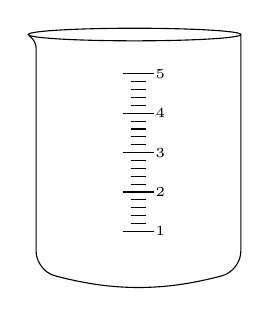
\begin{tikzpicture}
      \beaker{0,0}{0}
    \end{tikzpicture}
    \caption{空烧杯}
  \end{center}
\end{figure}
 
\begin{figure}[h!]
  \begin{center}
    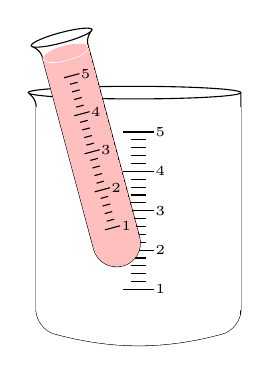
\begin{tikzpicture}
      \beaker{0,0}{1.00}
      \testtube[rotate={15},fill=red!25]{-0.2,0.8}{1.00}
    \end{tikzpicture}
    \caption{试管与烧杯}
  \end{center}
\end{figure}
 
\begin{figure}[h!]
  \begin{center}
    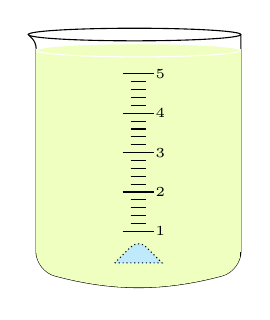
\begin{tikzpicture}
      \begin{scope}[shift={(0,0)}]
        \beaker[fill=lime!25]{0,0}{1.00}
        \pile[fill=cyan!25]{0,0}
      \end{scope}
    \end{tikzpicture}
    \caption{粉堆与烧杯}
  \end{center}
\end{figure}
 
\begin{figure}[h!]
  \begin{center}
    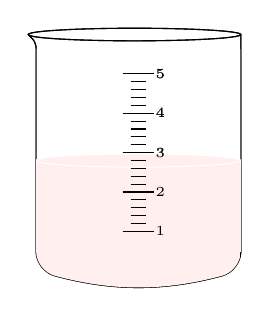
\begin{tikzpicture}
      \begin{scope}[shift={(0,0)}]
        \beaker{0,0}{1.00}
        \beaker[fill=pink!25]{0,0}{0.50}
      \end{scope}
    \end{tikzpicture}
    \caption{混合物与烧杯}
  \end{center}
\end{figure}
 
\begin{figure}[h!]
  \begin{center}
    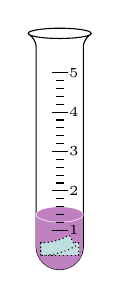
\begin{tikzpicture}
      \testtube[fill=violet!50]{0,0}{0.25}
      \metalcoil[fill=teal!25, scale=0.8]{0,0.1}
    \end{tikzpicture}
    \caption{有金属试剂的试管(25\%)}
  \end{center}
\end{figure}
 
\begin{figure}[h!]
  \begin{center}
    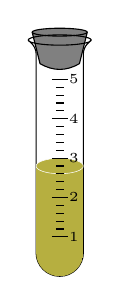
\begin{tikzpicture}
      \stopper{0,\testtubeheight}
      \testtube[fill=olive!65]{0,0}{0.50}      
    \end{tikzpicture}
    \caption{带塞子的试管{50\%}}
  \end{center}
\end{figure}

\begin{figure}[h!]
  \begin{center}
    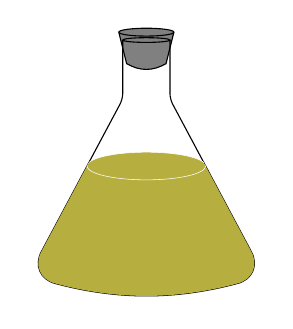
\begin{tikzpicture}
      \stopper{0,\testtubeheight}
      \erlenmeyer[fill=olive!65]{0,0}{0.50}      
    \end{tikzpicture}
    \caption{带塞子的锥形瓶{50\%}}
  \end{center}
\end{figure}

% 空的锥形瓶
\begin{figure}[h!]
  \begin{center}
    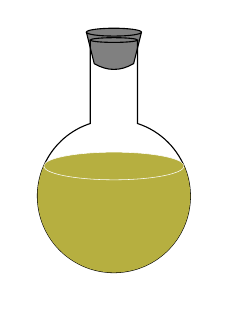
\begin{tikzpicture}
      \stopper{0,\testtubeheight}
      \ballon[fill=olive!65]{0,0}{0.50}      
    \end{tikzpicture}
    \caption{带塞子的球形瓶{50\%}}
  \end{center}
\end{figure}
 
\begin{figure}[h!]
  \begin{center}
    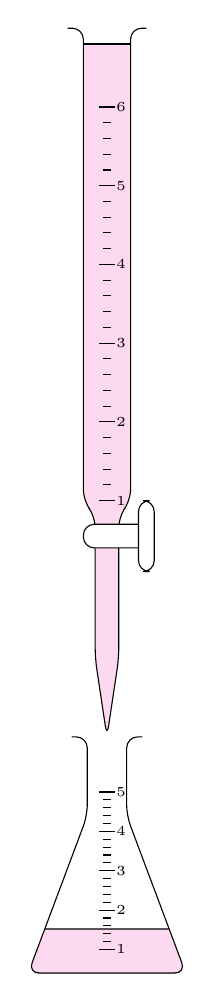
\begin{tikzpicture}
      \tikzstyle{glassware} = [fill=magenta!15]
      \flask{0,0}{0.2}
      \burette{0,3}{1.0}
    \end{tikzpicture}
    \caption{滴定管与锥形瓶}
    \label{d1}
  \end{center}
\end{figure}

\begin{figure}[h!]
  \begin{center}
    \begin{tikzpicture}
      \dropper[rotate={-45}]{0,0}
    \end{tikzpicture}
    \caption{滴管}
  \end{center}
\end{figure}

\begin{figure}[h!]
  \begin{center}
    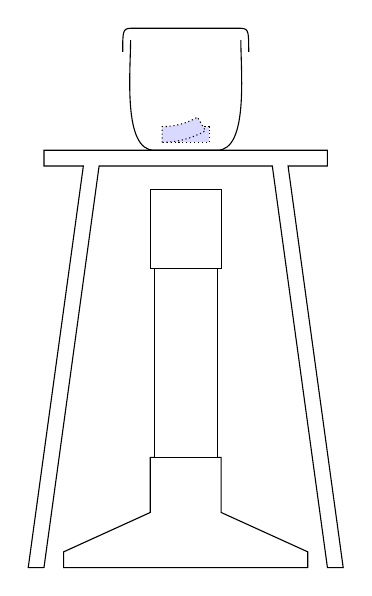
\begin{tikzpicture}
      \bunsen{0,0}
      \tripod{0,0}
      \crucible{0, \tripodheight}
      \cruciblelid{0,\tripodheight}
      \metalcoil[fill=blue!15]{0,\tripodheight}
    \end{tikzpicture}
    \caption{本生灯, 三角架, 带盖坩锅, 金属试剂}
  \end{center}
\end{figure}
 
\end{document}

%%% Local Variables:
%%% mode: latex
%%% TeX-master: t
%%% End:
